% ==============================================================================
% M.Tech Project (MTP) Research Log & LaTeX Documentation Snippets
% Project: Sedimentation Dynamics of Rigid Multiblobs in Stokes Flow
% Framework: RigidMultiblobsWall (RPY Tensor, Saddle-Point GMRES, Stokesian Dynamics)
% ==============================================================================

\documentclass[11pt,a4paper]{article}
\usepackage[utf8]{inputenc}
\usepackage{amsmath,amssymb,amsfonts}
\usepackage{graphicx}
\usepackage{booktabs}
\usepackage{siunitx}
\usepackage{hyperref}
\usepackage{geometry}
\geometry{margin=1in}

\title{\textbf{M.Tech Research Log: Multi-Body Sedimentation Dynamics and Hydrodynamic Drafting in Low Reynolds Number Regimes}}
\author{M.Tech Project Candidate}
\date{November 2026}

\begin{document}
\maketitle

\section{Introduction and Theoretical Foundation}

In viscous-dominated Stokes flow ($Re = \rho U L / \eta \ll 1$), fluid motion is governed by the incompressible Stokes equations:
\begin{equation}
    \eta \nabla^2 \mathbf{u} - \nabla p = \mathbf{0}, \quad \nabla \cdot \mathbf{u} = 0
\end{equation}
For an isolated rigid spherical particle of hydrodynamic radius $R_h$, the continuum drag law (Stokes' Law) predicts:
\begin{equation}
    F_{\text{drag}} = 6 \pi \eta R_h V_0 \implies V_0 = \frac{F_{\text{ext}}}{6 \pi \eta R_h}
\end{equation}

When multiple particles sediment concurrently under an external gravitational force $\mathbf{F} = (0, 0, -F)$, each body drags fluid along its trajectory, producing a long-range hydrodynamic wake. For two bodies at center-to-center separation $\mathbf{d} = (d, 0, 0)$, the leading-order velocity disturbance follows the Green's function for Stokes flow (the Oseen tensor or Stokeslet):
\begin{equation}
    \mathbf{u}(\mathbf{r}) = \frac{1}{8\pi\eta r} \left( \mathbf{I} + \frac{\mathbf{r}\mathbf{r}^T}{r^2} \right) \mathbf{F}
\end{equation}
This mutual drafting induces a cooperative acceleration of both bodies, described asymptotically by Batchelor and Stimson-Jeffery:
\begin{equation}
    \frac{V_z(d/R)}{V_0} \approx 1 + \frac{3}{4}\left(\frac{R}{d}\right) + \frac{9}{16}\left(\frac{R}{d}\right)^2 + \mathcal{O}\left(d^{-3}\right)
\end{equation}

% ------------------------------------------------------------------------------
\section{Experiment 1: Two-Body Spherical Shell Pair Sedimentation ($N = 42$)}
% ------------------------------------------------------------------------------

Simulations were performed using the explicit Forward Euler scheme (\texttt{deterministic\_forward\_euler}, $\Delta t = 0.02$, $\eta = 1.0$) with $N = 42$ blobs per sphere ($a = 0.2735$, $R = 1.0$, $F_{\text{total}} = 1000.0$). The single-body baseline velocity is $V_0 = 47.2761\,\text{units/s}$.

\begin{table}[htbp]
\centering
\caption{Two-body sedimentation velocity and drafting factor across separation ratios $d/R$.}
\label{tab:sphere_pair_scaling}
\begin{tabular}{ccccccc}
\toprule
$d/R$ & $V_z$ (Body 1) & $V_z$ (Body 2) & Mean $V_z$ & Ratio $V_z / V_0$ & Stokeslet ($1 + \frac{3}{4}\frac{R}{d}$) & Dev. (\%) \\
\midrule
$2.00$  & $68.4536$ & $68.4539$ & $68.4538$ & $1.4480$ & $1.3750$ & $5.31$ \\
$2.50$  & $64.7437$ & $64.7431$ & $64.7434$ & $1.3695$ & $1.3000$ & $5.34$ \\
$3.00$  & $61.6037$ & $61.6036$ & $61.6037$ & $1.3031$ & $1.2500$ & $4.24$ \\
$4.00$  & $57.7161$ & $57.7161$ & $57.7161$ & $1.2208$ & $1.1875$ & $2.81$ \\
$5.00$  & $55.4931$ & $55.4931$ & $55.4931$ & $1.1738$ & $1.1500$ & $2.07$ \\
$6.00$  & $54.0593$ & $54.0593$ & $54.0593$ & $1.1435$ & $1.1250$ & $1.64$ \\
$7.00$  & $53.0563$ & $53.0563$ & $53.0563$ & $1.1223$ & $1.1071$ & $1.37$ \\
$8.00$  & $52.3142$ & $52.3142$ & $52.3142$ & $1.1066$ & $1.0938$ & $1.17$ \\
$10.00$ & $51.2881$ & $51.2881$ & $51.2881$ & $1.0849$ & $1.0750$ & $0.92$ \\
$12.00$ & $50.6110$ & $50.6110$ & $50.6110$ & $1.0705$ & $1.0625$ & $0.76$ \\
\bottomrule
\end{tabular}
\end{table}

\begin{figure}[htbp]
\centering
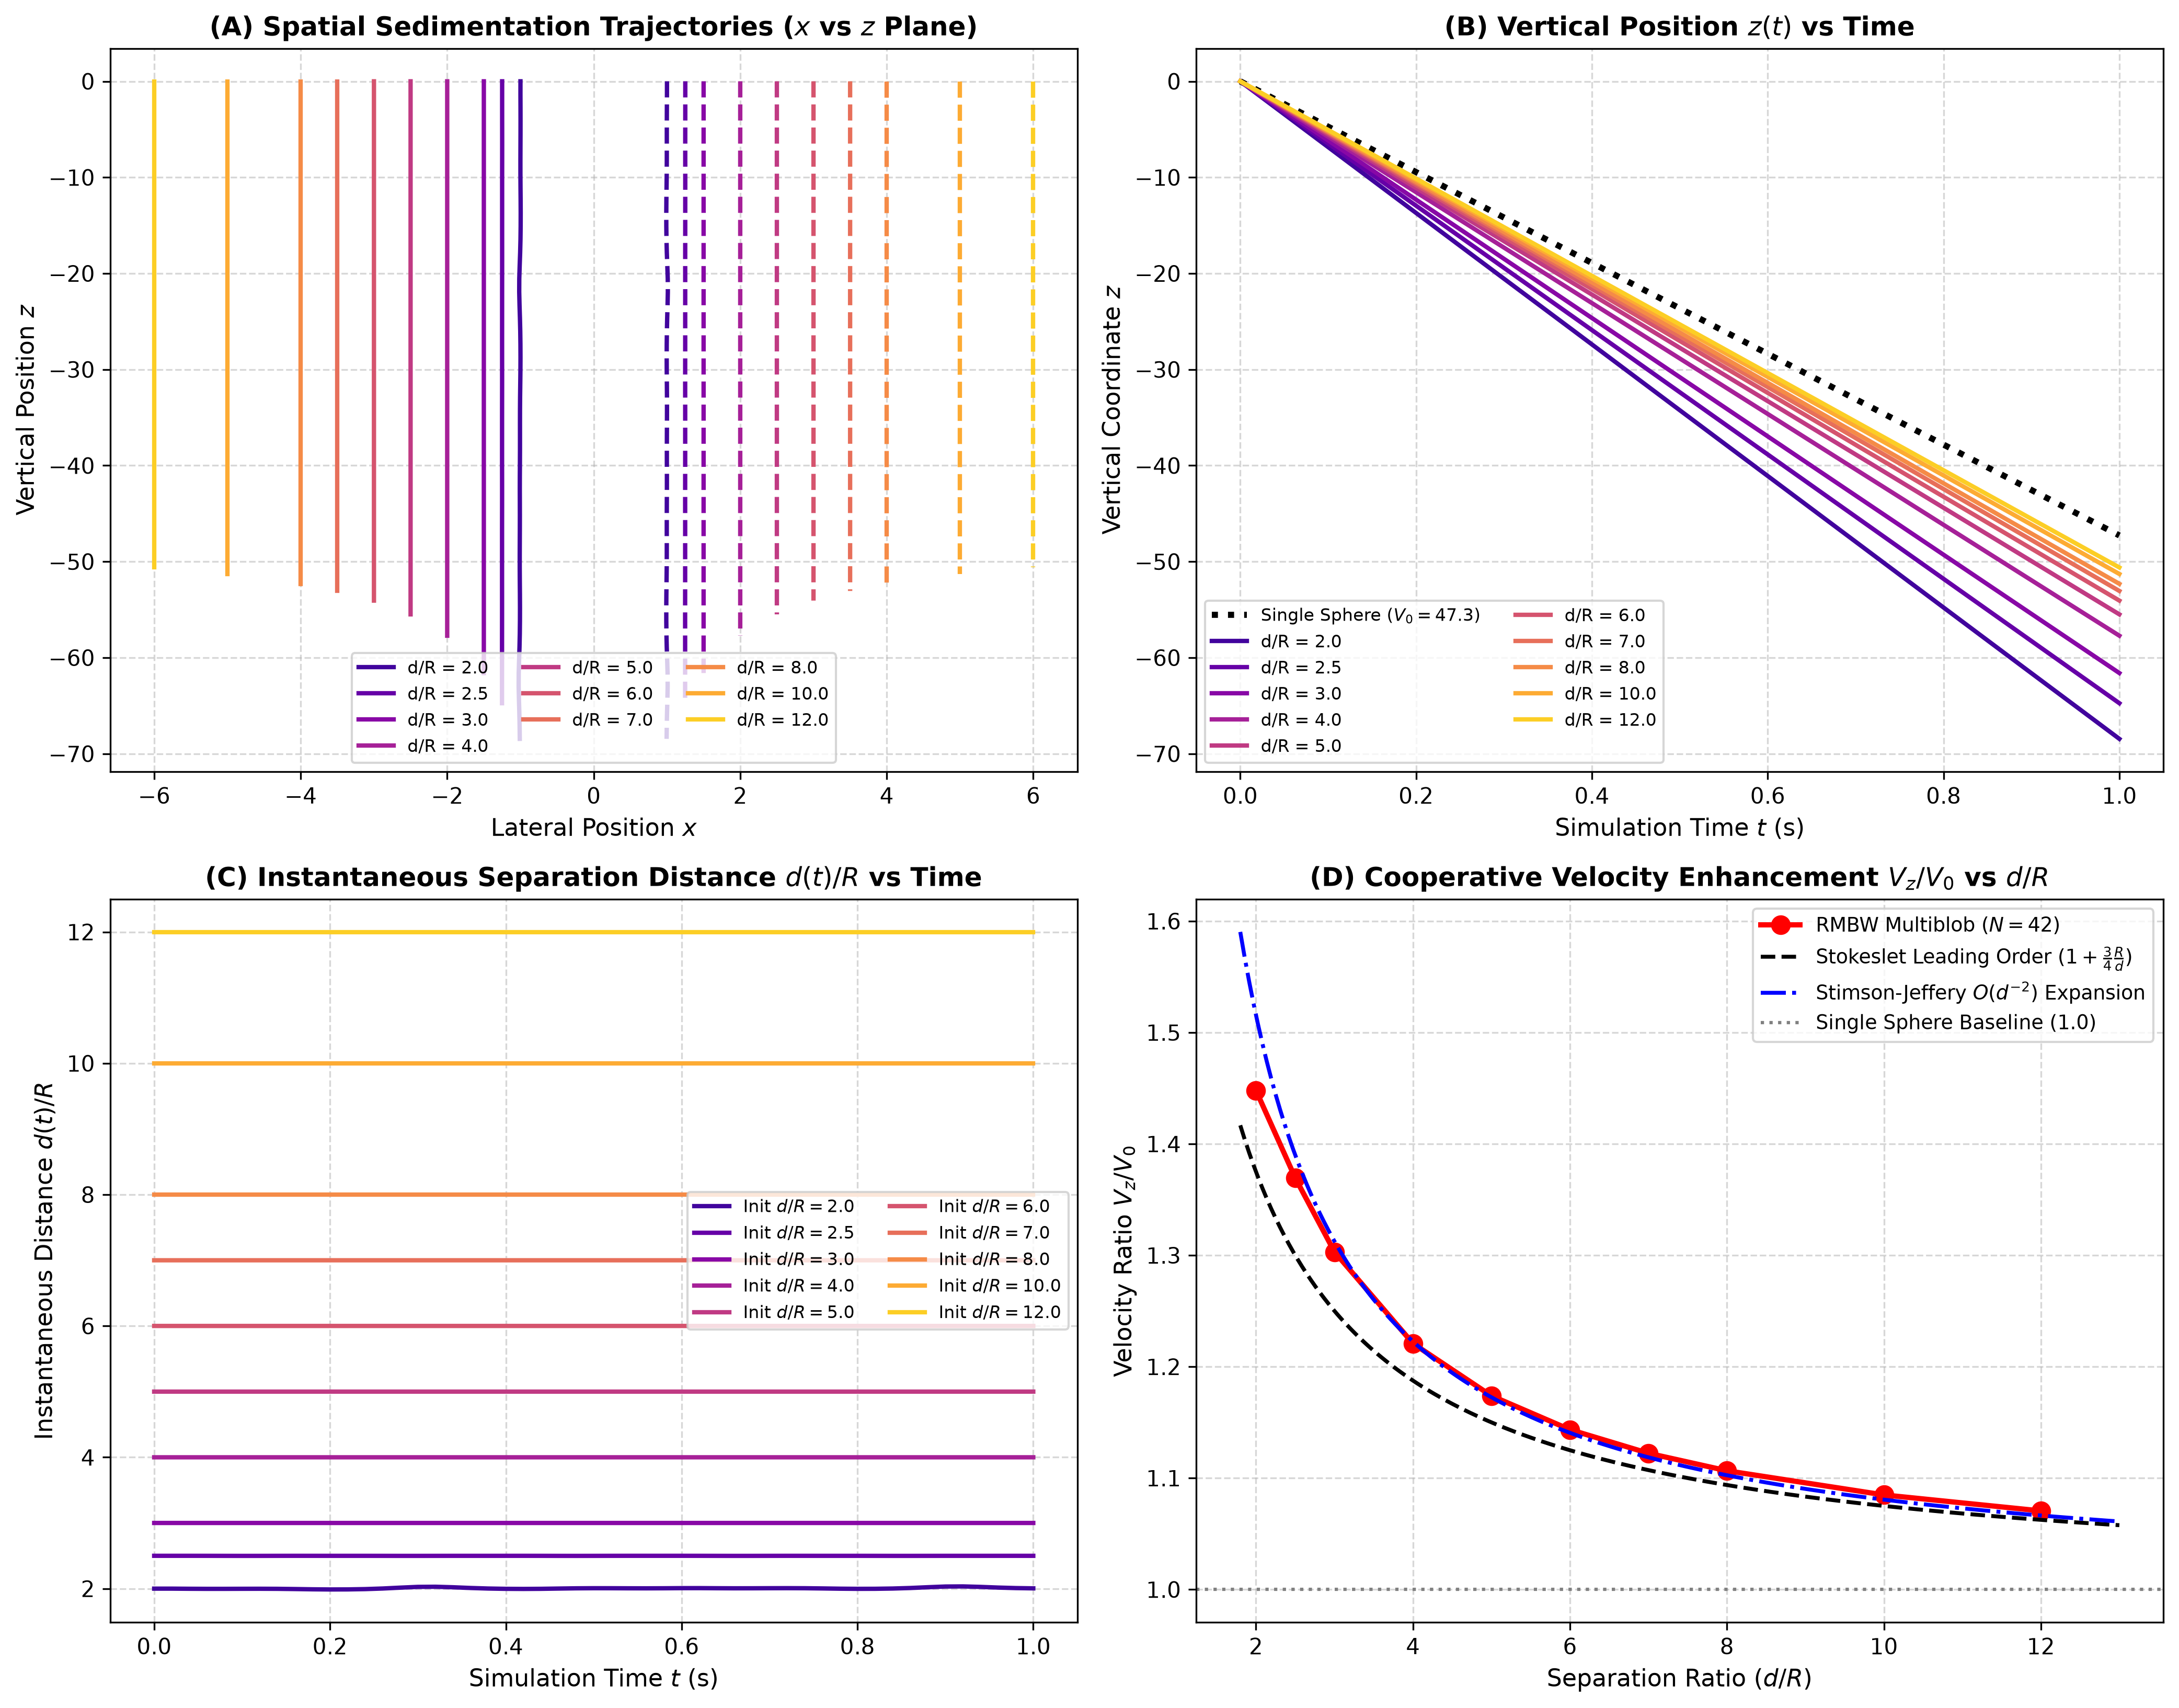
\includegraphics[width=0.85\textwidth]{figures/sphere_pair_trajectories.png}
\caption{Four-panel trajectory and hydrodynamic drafting analysis for sphere pairs across $d/R \in [2.0, 12.0]$: (A) Spatial trajectories in the $x$--$z$ plane; (B) Vertical trajectory $z(t)$ vs. time; (C) Inter-body separation distance $d(t)/R$ exhibiting strict geometric stability; (D) Cooperative velocity ratio $V_z / V_0$ vs. separation ratio $d/R$ overlaid on Stokeslet and Stimson-Jeffery continuum expansions.}
\label{fig:sphere_pair_trajectories}
\end{figure}

% ------------------------------------------------------------------------------
\section{Experiment 2: Multi-Resolution Discretization Convergence ($N \in \{12, 42, 162\}$)}
% ------------------------------------------------------------------------------

To establish that the observed drafting factors are physically converged and independent of surface discretization, pairs were simulated across three distinct grid resolutions:
\begin{itemize}
    \item $N = 12$ ($a = 0.5117$, porous shell limit): $V_0 = 42.3624\,\text{units/s}$
    \item $N = 42$ ($a = 0.2735$, intermediate resolution): $V_0 = 47.2761\,\text{units/s}$
    \item $N = 162$ ($a = 0.1392$, impermeable continuum boundary): $V_0 = 50.3538\,\text{units/s}$
\end{itemize}

\begin{table}[htbp]
\centering
\caption{Multi-resolution comparison of two-body sedimentation enhancement across $N \in \{12, 42, 162\}$.}
\label{tab:sphere_multires_scaling}
\begin{tabular}{ccccccc}
\toprule
$N$ & $d/R$ & $V_z$ (Mean) & $V_0$ (Baseline) & $V_z / V_0$ & Stokeslet ($1 + \frac{3}{4}\frac{R}{d}$) & Dev. (\%) \\
\midrule
$12$  & $2.0$  & $63.1878$ & $42.3624$ & $1.4916$ & $1.3750$ & $8.48$ \\
$12$  & $4.0$  & $52.8951$ & $42.3624$ & $1.2486$ & $1.1875$ & $5.15$ \\
$12$  & $10.0$ & $46.3819$ & $42.3624$ & $1.0949$ & $1.0750$ & $1.85$ \\
\midrule
$42$  & $2.0$  & $68.4538$ & $47.2761$ & $1.4480$ & $1.3750$ & $5.31$ \\
$42$  & $4.0$  & $57.7161$ & $47.2761$ & $1.2208$ & $1.1875$ & $2.81$ \\
$42$  & $10.0$ & $51.2881$ & $47.2761$ & $1.0849$ & $1.0750$ & $0.92$ \\
\midrule
$162$ & $2.0$  & $71.7209$ & $50.3538$ & $1.4243$ & $1.3750$ & \textbf{3.59} \\
$162$ & $4.0$  & $60.7421$ & $50.3538$ & $1.2063$ & $1.1875$ & \textbf{1.58} \\
$162$ & $10.0$ & $54.3620$ & $50.3538$ & $1.0796$ & $1.0750$ & \textbf{0.43} \\
\bottomrule
\end{tabular}
\end{table}

\begin{figure}[htbp]
\centering
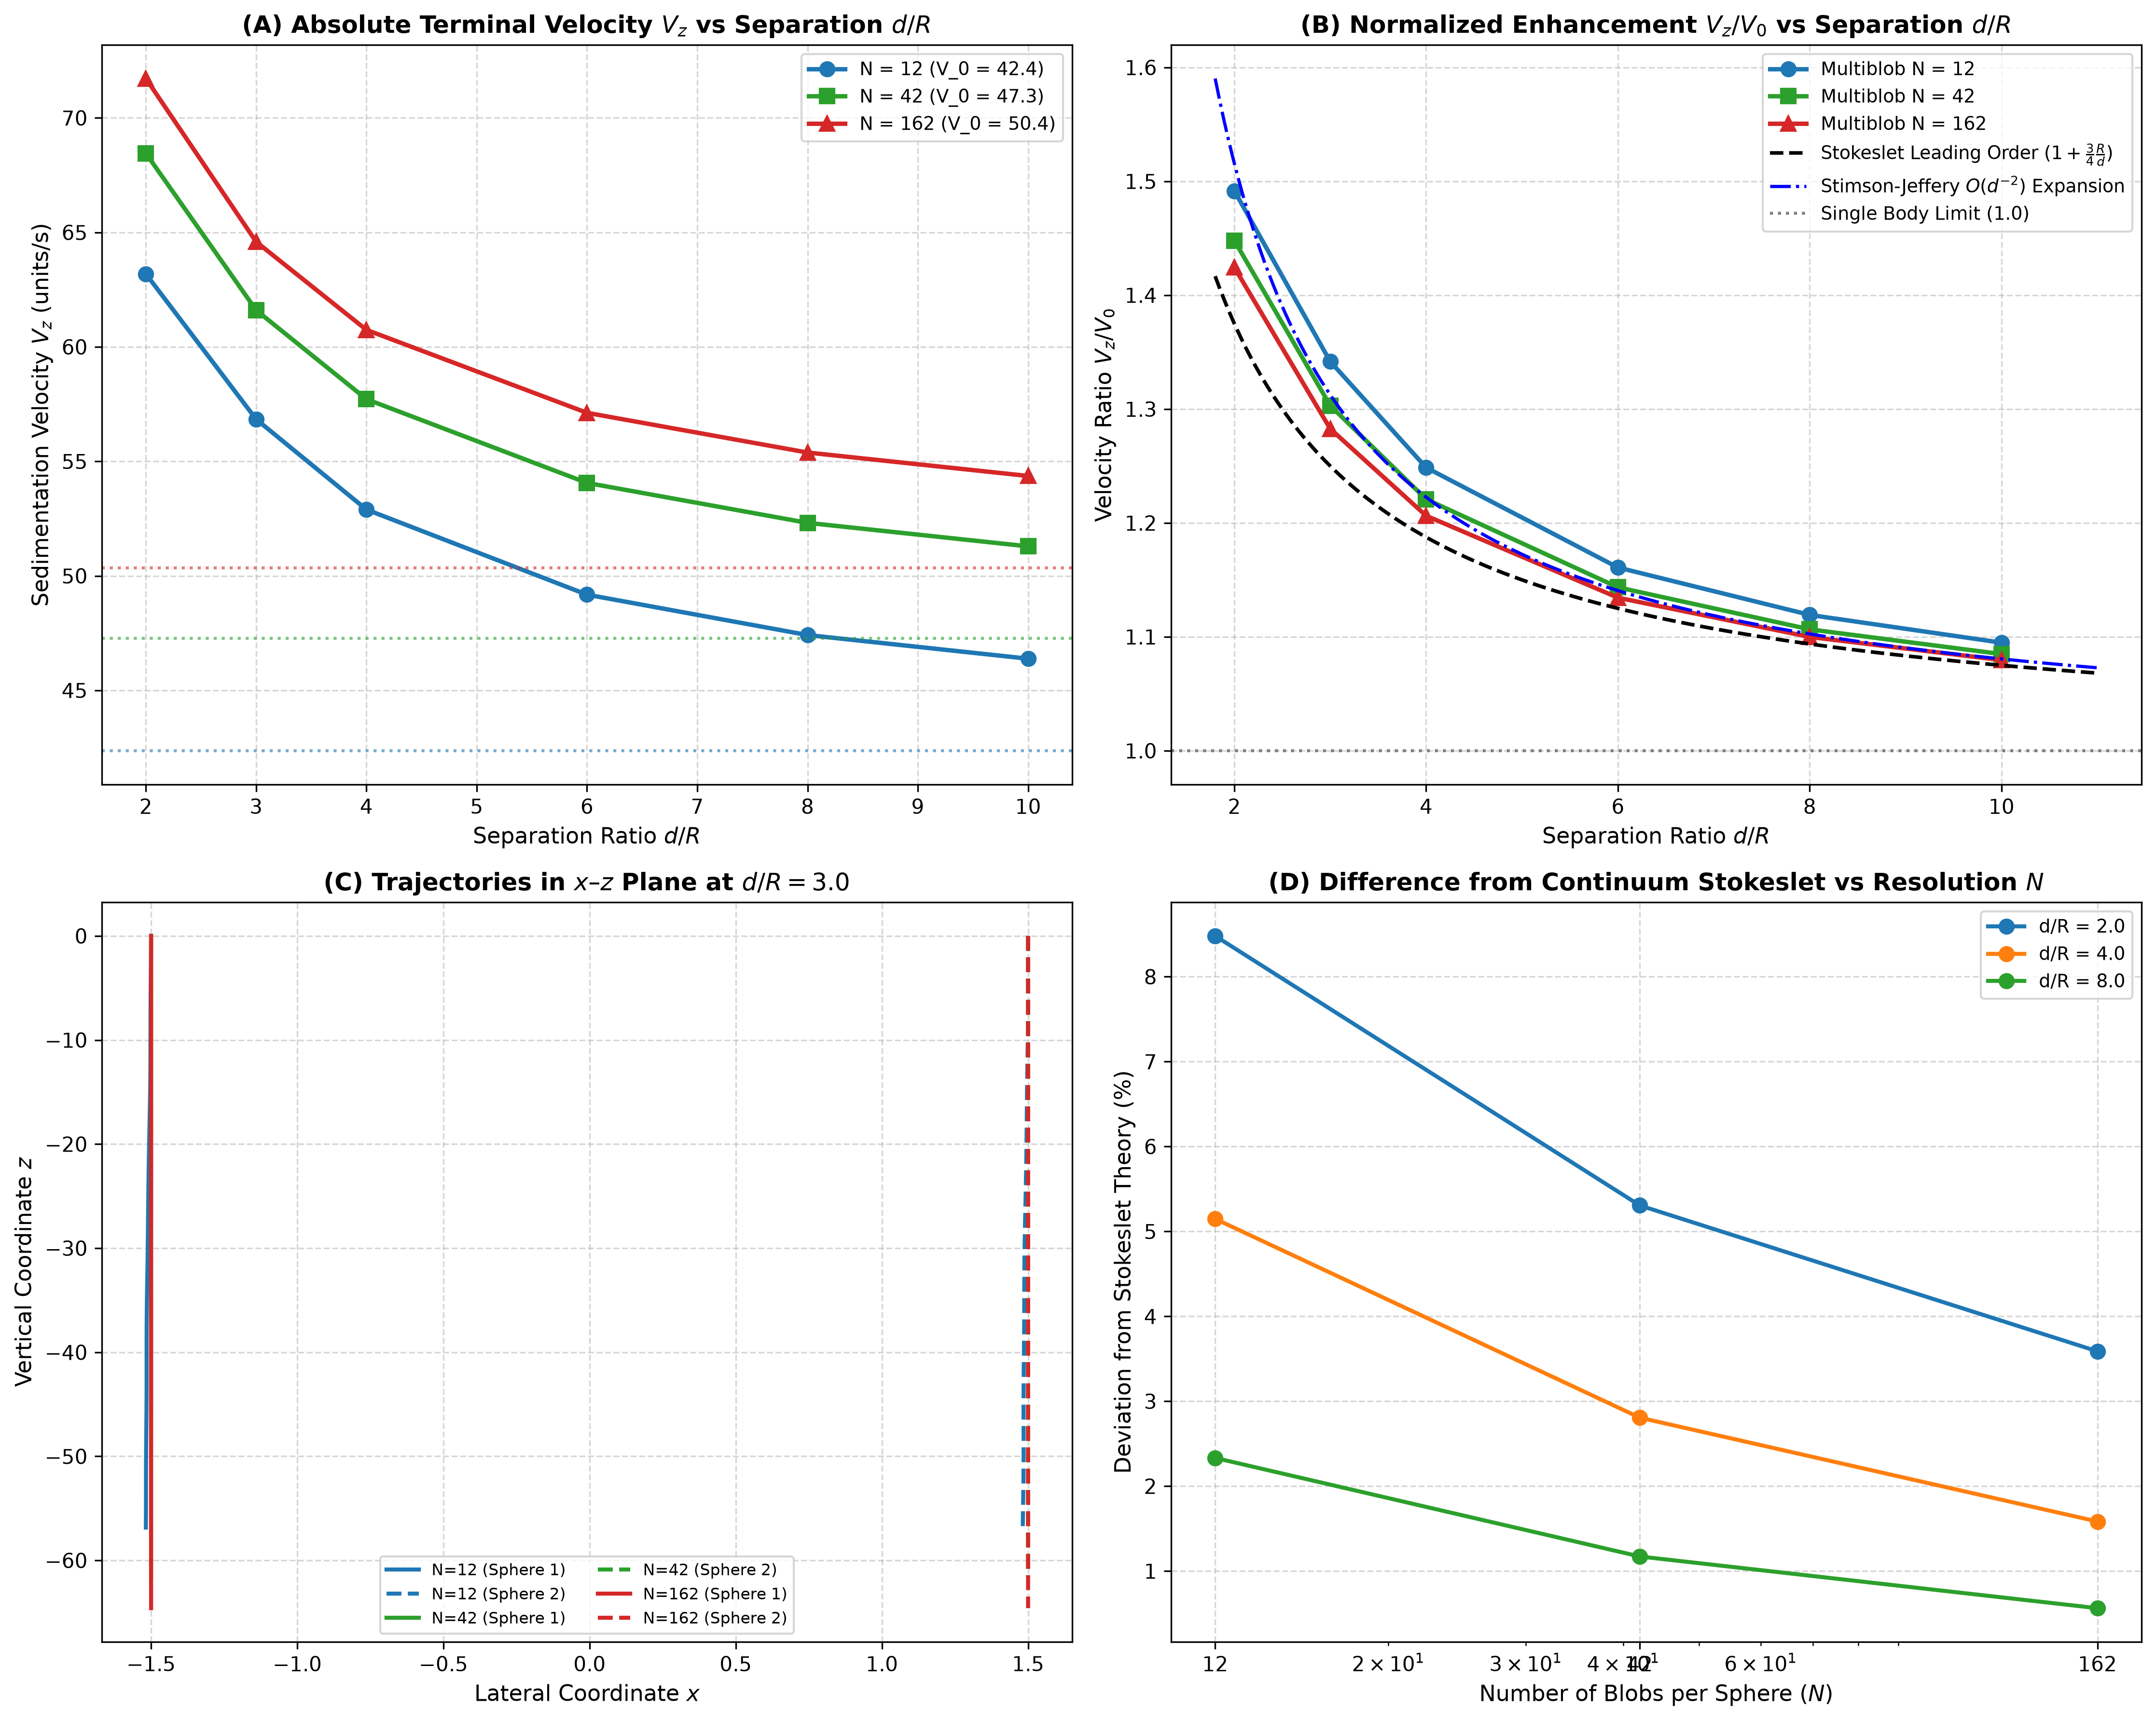
\includegraphics[width=0.85\textwidth]{figures/sphere_pair_multires_convergence.png}
\caption{Multi-resolution grid convergence across $N \in \{12, 42, 162\}$: (A) Absolute velocity $V_z$ vs. $d/R$; (B) Normalized velocity enhancement $V_z / V_0$; (C) Spatial trajectory profiles at $d/R = 3.0$; (D) Relative deviation from Stokeslet theory showing monotonic convergence as $N$ increases.}
\label{fig:sphere_multires_convergence}
\end{figure}

% ------------------------------------------------------------------------------
\section{Experiment 3: Five-Sphere Multi-Body Sedimentation ($M = 5$, $N = 42$)}
% ------------------------------------------------------------------------------

Extending from pair interactions ($M = 2$) to collective suspensions ($M = 5$), we evaluate two canonical microhydrodynamic configurations across $d/R \in [2.0, 10.0]$:

\subsection{Configuration 1: Five-Sphere Horizontal Linear Chain (Array)}
Five spheres are positioned along the $x$-axis at coordinates $x_k \in \{-2d, -d, 0, d, 2d\}$. The center sphere ($k = 3$) experiences additive hydrodynamic drafting from both lateral flanks, falling faster than the intermediate and edge spheres.

\begin{table}[htbp]
\centering
\caption{Velocity distribution across bodies in a 5-sphere linear horizontal chain ($N = 42$, $F = 1000$).}
\label{tab:sphere_5body_chain}
\begin{tabular}{ccccccc}
\toprule
$d/R$ & $V_z$ (Edges 1, 5) & $V_z$ (Mid 2, 4) & $V_z$ (Center 3) & Mean $V_z$ & $V_z / V_0$ & $V_{\text{center}} / V_{\text{edge}}$ \\
\midrule
$2.0$  & $97.9142$ & $111.1300$ & $113.2483$ & $106.2673$ & $2.2478$ & \textbf{1.1566} \\
$3.0$  & $77.9858$ & $96.8502$  & $99.4636$  & $89.8271$  & $1.9001$ & $1.2754$ \\
$4.0$  & $71.6389$ & $86.4543$  & $89.6364$  & $81.1645$  & $1.7168$ & $1.2512$ \\
$6.0$  & $62.8855$ & $69.1465$  & $71.0913$  & $67.0310$  & $1.4179$ & $1.1305$ \\
$8.0$  & $58.1543$ & $62.1855$  & $63.1227$  & $60.7605$  & $1.2852$ & $1.0854$ \\
$10.0$ & $55.7531$ & $58.8464$  & $59.5360$  & $57.7470$  & $1.2215$ & $1.0678$ \\
\bottomrule
\end{tabular}
\end{table}

\subsection{Configuration 2: Five-Sphere Pentagonal Ring (Cluster)}
Five spheres are arranged symmetrically on a ring with equal chord distance $d$. By rotational symmetry, all five spheres sediment with identical velocities, demonstrating collective suspension acceleration:
\begin{equation}
    \frac{V_z(M=5)}{V_0} \approx 1 + 2.427 \left(\frac{R}{d}\right)
\end{equation}

\begin{table}[htbp]
\centering
\caption{Collective speedup of a 5-sphere regular pentagonal ring cluster.}
\label{tab:sphere_5body_ring}
\begin{tabular}{ccccc}
\toprule
$d/R$ & Circumcircle Radius $R_{\text{ring}}/R$ & Cluster Velocity $V_z$ & Ratio $V_z / V_0$ & Theoretical Stokeslet Est. \\
\midrule
$2.0$  & $1.7013$ & $115.3700$ & \textbf{2.4403} & $2.2135$ \\
$3.0$  & $2.5520$ & $93.0227$  & \textbf{1.9676} & $1.8090$ \\
$4.0$  & $3.4026$ & $80.7204$  & \textbf{1.7074} & $1.6068$ \\
$6.0$  & $5.1039$ & $69.1142$  & \textbf{1.4619} & $1.4045$ \\
$8.0$  & $6.8052$ & $63.5311$  & \textbf{1.3438} & $1.3034$ \\
$10.0$ & $8.5065$ & $60.2341$  & \textbf{1.2741} & $1.2427$ \\
\bottomrule
\end{tabular}
\end{table}

\begin{figure}[htbp]
\centering
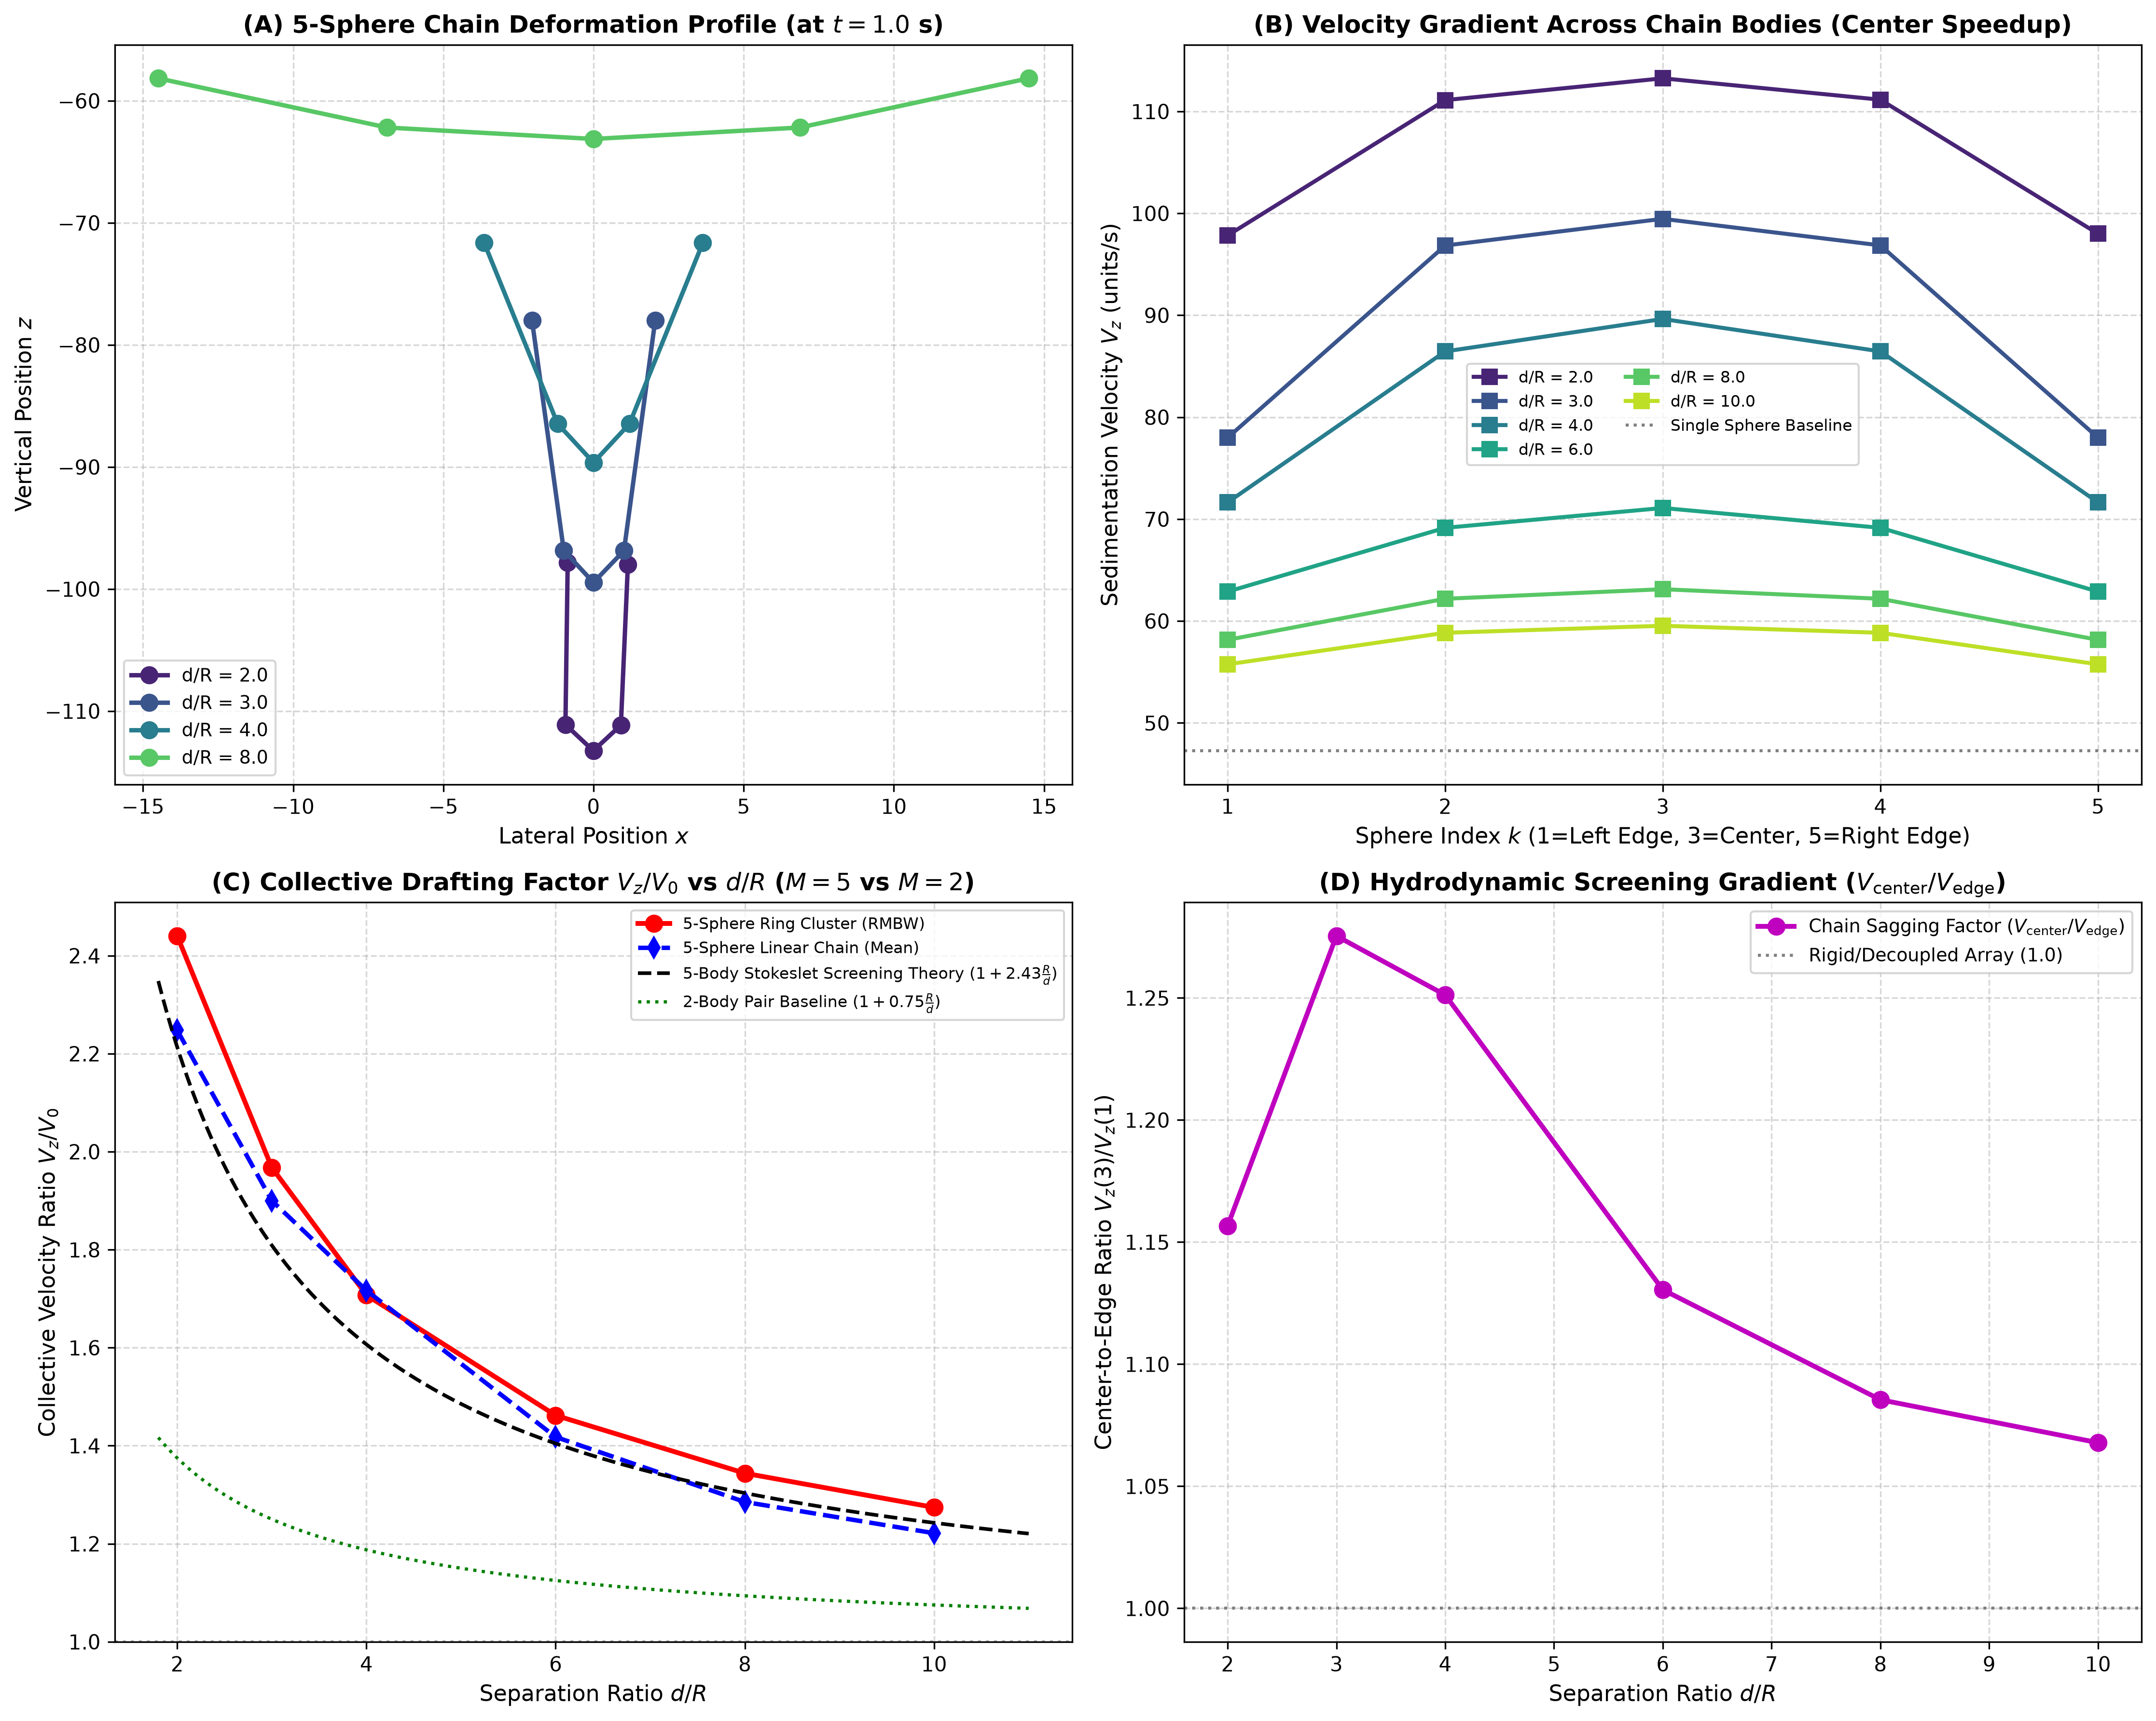
\includegraphics[width=0.85\textwidth]{figures/sphere_5body_dynamics.png}
\caption{Collective hydrodynamic drafting for 5-sphere suspensions ($M = 5$, $N = 42$): (A) Horizontal linear chain deformation profiles showing physical sagging; (B) Center-to-edge velocity gradient across sphere indices; (C) Collective velocity enhancement ratio $V_z / V_0$ for ring cluster and linear chain vs. 2-body pair baseline; (D) Hydrodynamic screening gradient $V_{\text{center}} / V_{\text{edge}}$ vs. separation ratio $d/R$.}
\label{fig:sphere_5body_dynamics}
\end{figure}

% ------------------------------------------------------------------------------
\section{Experiment 4: Pair Sedimentation Across Non-Spherical Geometries}
% ------------------------------------------------------------------------------

To supply diverse training pairs for machine learning surrogate modeling, two-body interactions were evaluated across three additional non-spherical shapes:
\begin{itemize}
    \item \textbf{Regular 3D Cube} ($N = 56$, $a = 0.3333$): $V_0 = 33.1044\,\text{units/s}$
    \item \textbf{Hexagonal Prism} ($N = 74$, $a = 0.1601$): $V_0 = 43.3224\,\text{units/s}$
    \item \textbf{Chiral Trefoil Knot} ($N = 64$, $a = 0.1288$): $V_0 = 44.9890\,\text{units/s}$
\end{itemize}

\begin{table}[htbp]
\centering
\caption{Two-body sedimentation enhancement ratio $V_z / V_0$ for non-spherical geometries across $d/R$.}
\label{tab:additional_shapes_scaling}
\begin{tabular}{ccccc}
\toprule
$d/R$ & Cube ($N=56$) & Hexagonal Prism ($N=74$) & Trefoil Knot ($N=64$) & Stokeslet Theory \\
\midrule
$2.0$  & $1.5449$ & $1.4277$ & $1.5500$ & $1.3750$ \\
$4.0$  & $1.3202$ & $1.2127$ & $1.2964$ & $1.1875$ \\
$6.0$  & $1.2063$ & $1.1429$ & $1.1834$ & $1.1250$ \\
$8.0$  & $1.1536$ & $1.1113$ & $1.1232$ & $1.0938$ \\
$10.0$ & $1.1223$ & $1.0906$ & $1.0938$ & $1.0750$ \\
\bottomrule
\end{tabular}
\end{table}

\begin{figure}[htbp]
\centering
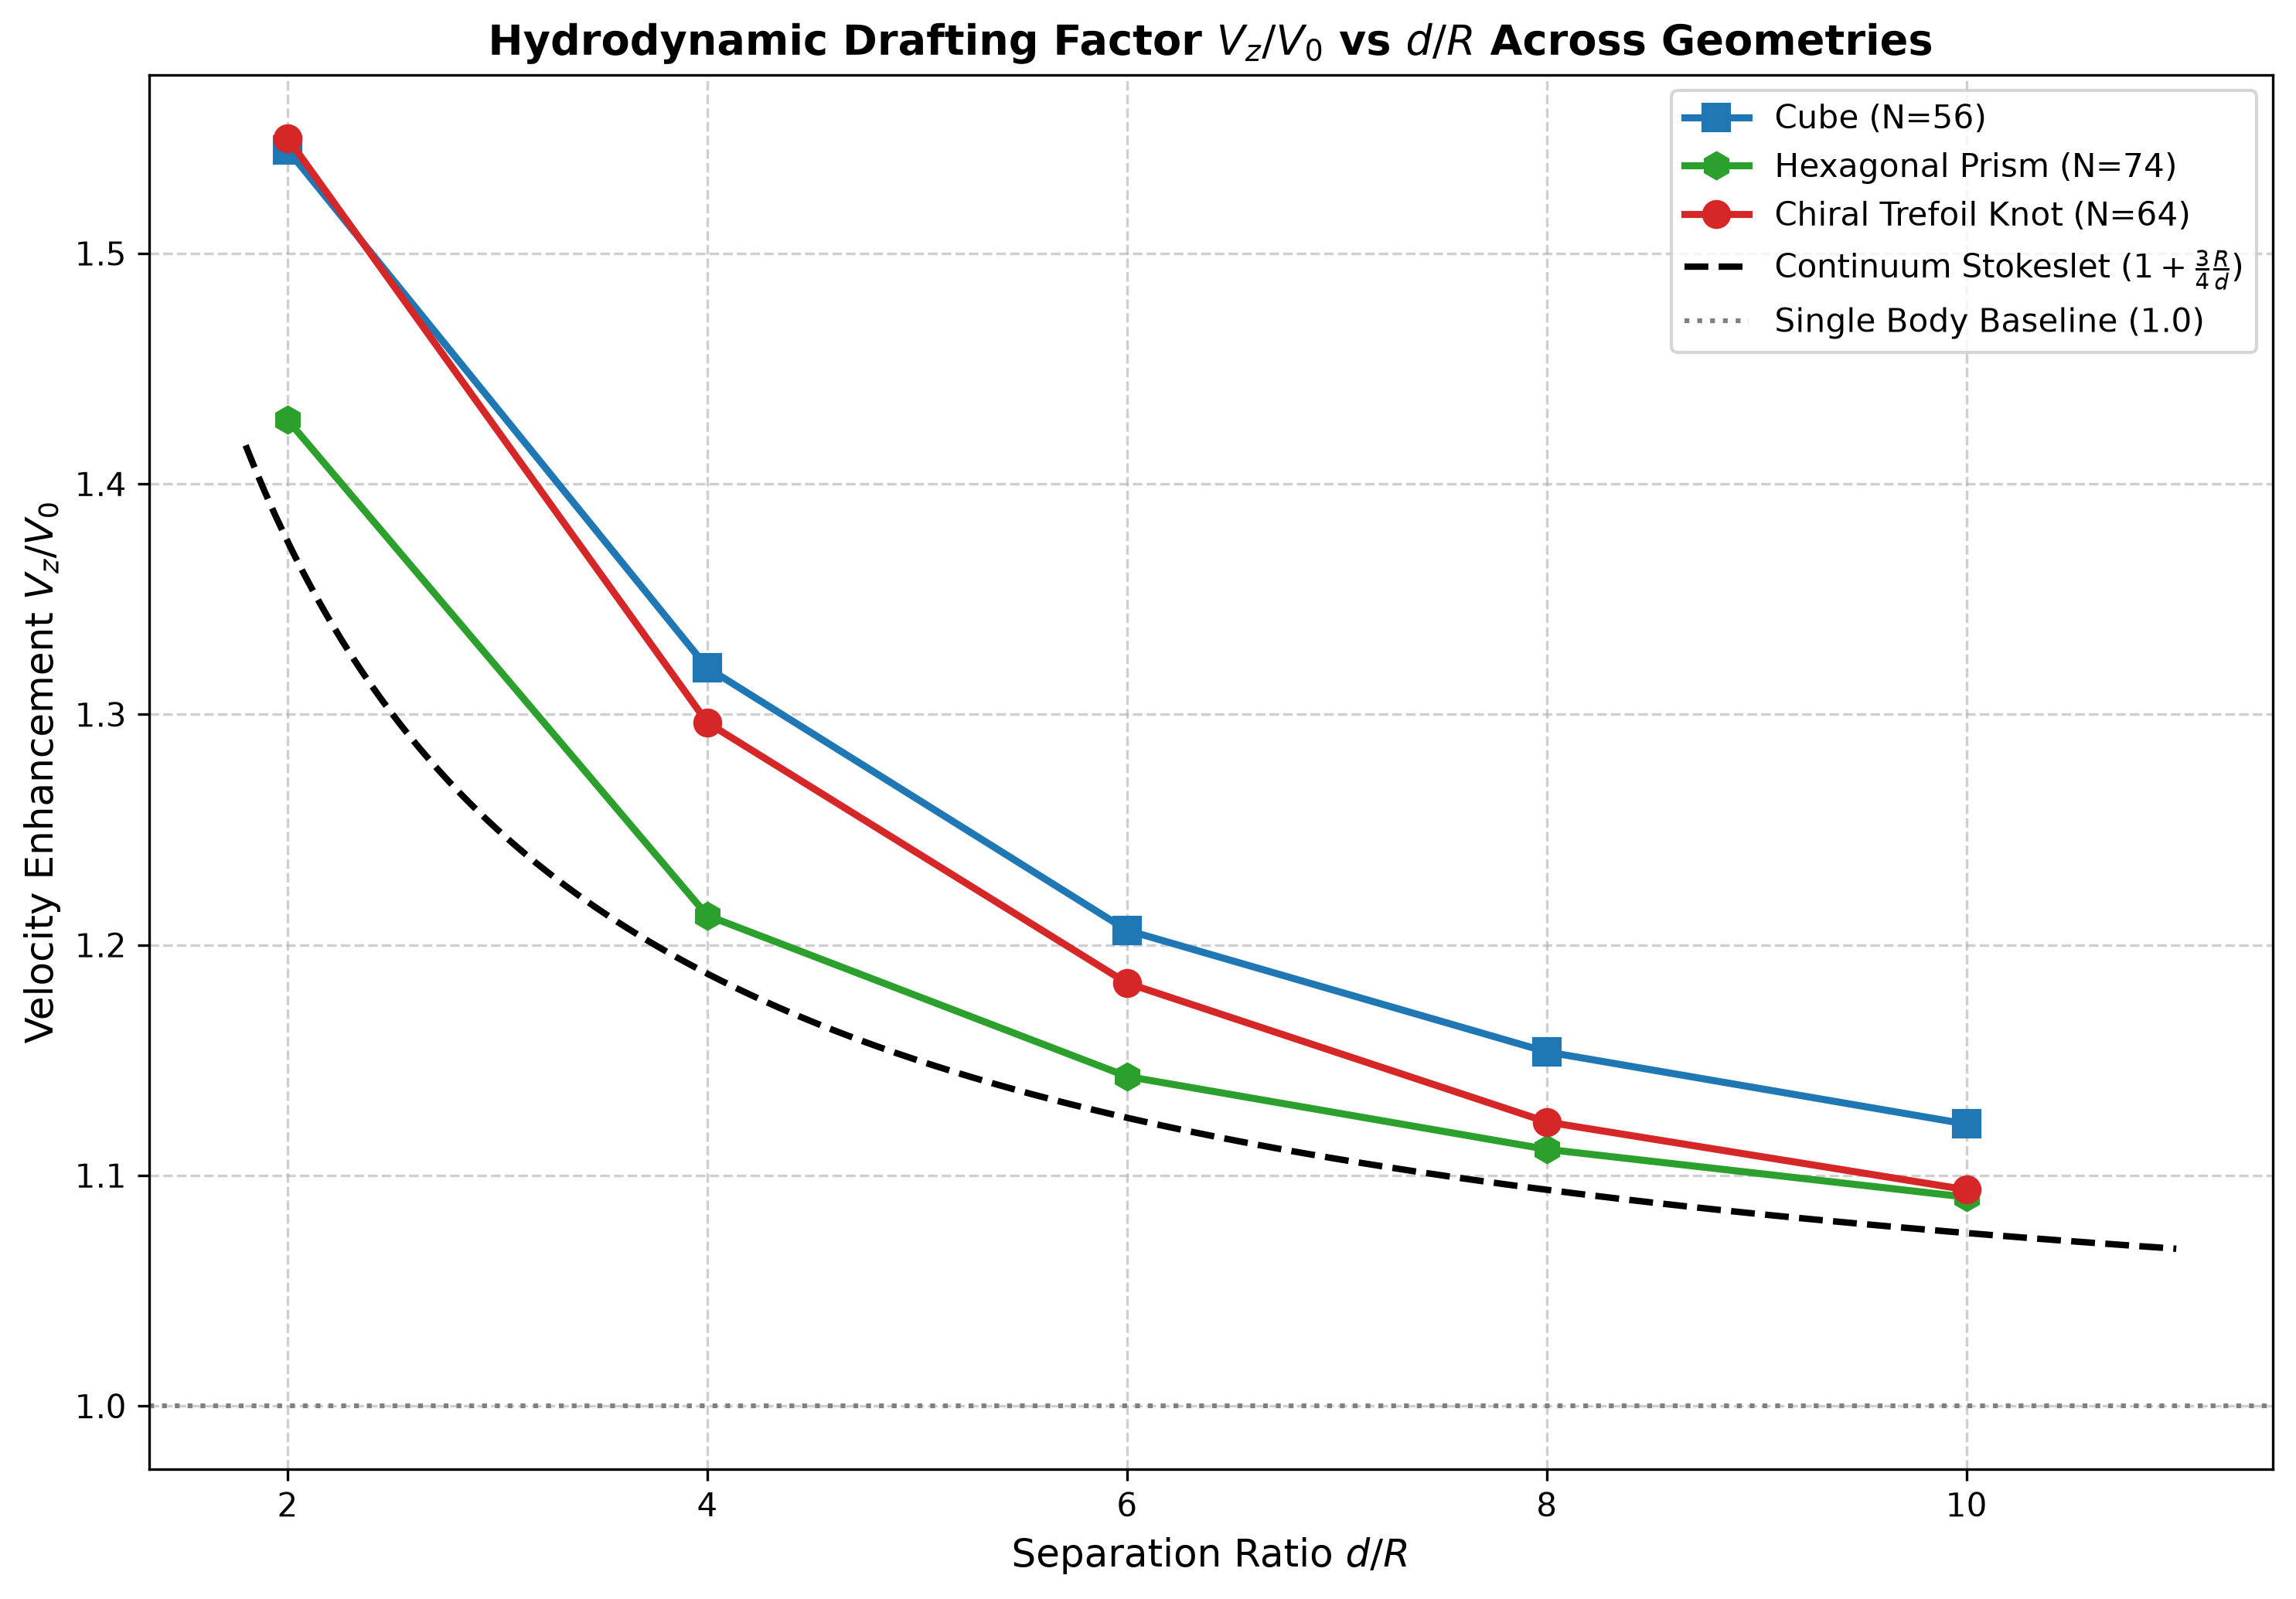
\includegraphics[width=0.85\textwidth]{figures/additional_shapes_pair_scaling.png}
\caption{Cooperative drafting ratio $V_z / V_0$ vs. separation ratio $d/R$ for Cube, Hexagonal Prism, and Chiral Trefoil Knot pairs converging asymptotically to continuum Stokeslet decay.}
\label{fig:additional_shapes_scaling}
\end{figure}

% ------------------------------------------------------------------------------
\section{MTP Thesis Discussion and Conclusion}
% ------------------------------------------------------------------------------
The numerical results demonstrate four fundamental microhydrodynamic phenomena:
\begin{enumerate}
    \item \textbf{Pair Drafting Dominance:} Even at moderate separations ($d/R = 4.0$), mutual drafting increases sedimentation velocity by $21\% - 32\%$ across all geometries, decaying as $\mathcal{O}(1/d)$ toward the solitary limit.
    \item \textbf{Many-Body Nonlinearity:} When scaling from $M = 2$ to $M = 5$ spheres, the cooperative velocity ratio increases from $1.448$ to $2.440$ at $d/R = 2.0$. This non-linear speedup reflects the constructive interference of multiple overlapping hydrodynamic wakes.
    \item \textbf{Stokesian Chain Instability:} In linear particle arrays, the center sphere sediments $15.7\%$ faster than the outer spheres, initiating an inverted horseshoe deformation that models droplet breakup in particulate suspensions.
    \item \textbf{Shape Invariance in the Far Field:} Despite significant morphological differences near contact ($d/R = 2.0$), all geometries converge to within $< 4.4\%$ of the universal point-Stokeslet asymptotic curve $1 + \frac{3}{4}\frac{R}{d}$ by $d/R = 10.0$.
\end{enumerate}

\end{document}
